\documentclass[border=3pt]{standalone}
% Preâmbulo compartilhado pelos diagramas TikZ da aula
\usepackage[T1]{fontenc}
\usepackage[utf8]{inputenc}
\usepackage{lmodern}
\usepackage{amsmath}
\usepackage{xcolor}
\usepackage{tikz}
\usetikzlibrary{arrows.meta,angles,quotes,decorations.pathmorphing,calc,
                positioning,shapes.geometric,backgrounds,fit}

% Paleta (mesma dos SVGs originais)
\definecolor{dblue}{HTML}{2A5B8C}
\definecolor{dorange}{HTML}{B3541E}
\definecolor{dgreen}{HTML}{4A7C59}
\definecolor{dred}{HTML}{9C4B4B}
\definecolor{dcream}{HTML}{F4F1EA}
\definecolor{dshade}{HTML}{DDD7C9}

% Estilos comuns (prefixo d... para não colidir com chaves internas do pgf)
\tikzset{
  >={Stealth[length=2mm]},
  dguide/.style={gray!55, dashed, line width=0.4pt},
  daxis/.style={gray!60, line width=0.7pt, ->},
  dbody/.style={fill=black!3, draw=black!80, line width=1pt},
  dacc/.style={draw=dblue, line width=1pt},
  dlbl/.style={black!55, font=\small},
  dsub/.style={black!45, font=\footnotesize},
  dstate/.style={circle, draw=black!80, fill=dcream, line width=1pt,
                 minimum size=17mm, font=\large, inner sep=1pt},
  dobs/.style={circle, draw=black!80, fill=dshade, line width=1pt,
               minimum size=14mm, font=\large, inner sep=1pt},
  dbox/.style={rounded corners=2pt, draw=black!80, fill=dcream, line width=1pt,
               align=center, inner sep=6pt},
  dtrans/.style={->, dblue, line width=1pt},
  dmeas/.style={->, dorange, line width=1pt},
}

\begin{document}
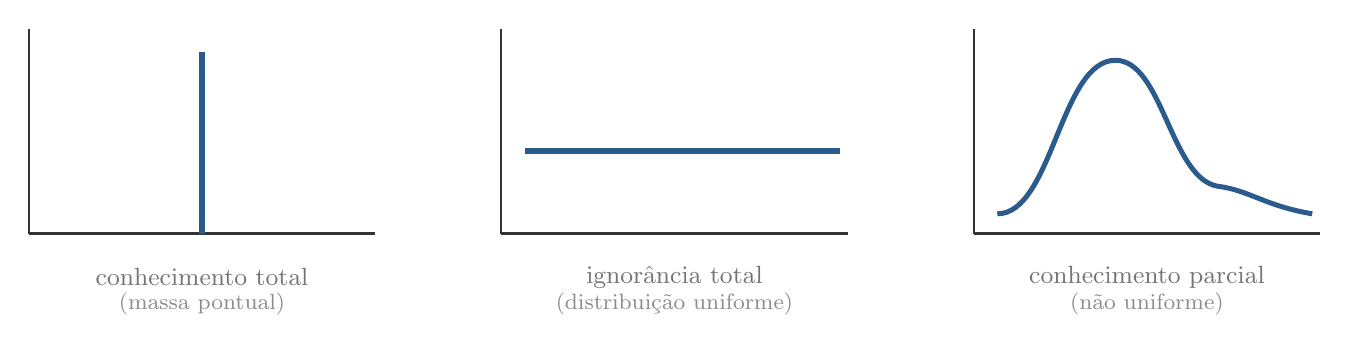
\begin{tikzpicture}[x=1cm,y=1cm]

  \foreach \dx/\lbl/\sub [count=\i] in {%
      0/{conhecimento total}/{(massa pontual)},
      6/{ignorância total}/{(distribuição uniforme)},
      12/{conhecimento parcial}/{(não uniforme)}}
  {
    \begin{scope}[shift={(\dx,0)}]
      \draw[black!80, line width=0.8pt] (0,0) -- (4.4,0);
      \draw[black!80, line width=0.8pt] (0,0) -- (0,2.6);
      \node[dlbl] at (2.2,-0.55) {\lbl};
      \node[dsub] at (2.2,-0.9)  {\sub};
    \end{scope}
  }

  % panel 1: massa pontual
  \draw[dblue, line width=2.2pt] (2.2,0) -- (2.2,2.3);

  % panel 2: uniforme
  \draw[dblue, line width=2.2pt] (6.3,1.05) -- (10.3,1.05);

  % panel 3: parcial (bimodal suave)
  \draw[dblue, line width=1.8pt]
    (12.3,0.25) .. controls (13.0,0.25) and (13.1,2.2) .. (13.8,2.2)
    .. controls (14.4,2.2) and (14.5,0.7) .. (15.1,0.6)
    .. controls (15.5,0.55) and (15.7,0.35) .. (16.3,0.25);

\end{tikzpicture}
\end{document}
